
\section{Evaluation}
\label{sec:evaluation}

We evaluated \sys{} on \xiangyu{one cluster consisting of }three machines. Server A is a dual-socket Intel Gold 6138 processor (80 cores, 2.0 GHz, 55 MB LLC) equipped with 256 GB DDR3 RAM and an NVIDIA P40 GPU. Server B is a single socket Intel Xeon 6787p (86 cores, 2.0 GHz, 336MB LLC) with 768 GB DDR5 RAM(512GB CXL Module) and an NVIDIA H100 GPU. Server C is a Grace Hopper Machine. Unless otherwise mentioned, each metric is the average of 10 trials on server A.\xiangyu{Why do we choose 10? Is 10 sufficient to prove the effectiveness? May be worthwhile to say it.}  We report averages using geometric mean for \xiangyu{metrics such as the average speedup and arithmetic mean for the rest}.

\xiangyu{I like your description in the eval section. To highlight our results, I suggest highlighting 1 sentence in each subsection.}

\subsection{Micro-benchmark Performance}

We quantify instrumentation overhead with a latency micro-benchmark that measures GPU load/store latency under \sys{} vs. NVBit (gpumemtrace~\cite{villa2019nvbit}) across varying access sizes. As shown in Figure~\ref{fig:end_to_end_latency}, \sys{} adds substantially less latency than NVBit, staying low and stable below 128 KB and rising modestly thereafter. \xiangyu{Do we need to say some numeric values? (e.g., A's latency is x times lower than B's)} \Cref{fig:latency1} compares with the PyTorch profiler (CUPTI+NVTX): p10 and mean latencies are slightly better under \sys{}. Lightweight PTX injection at runtime is the key enabler of the lower overhead.

\begin{figure} \centering 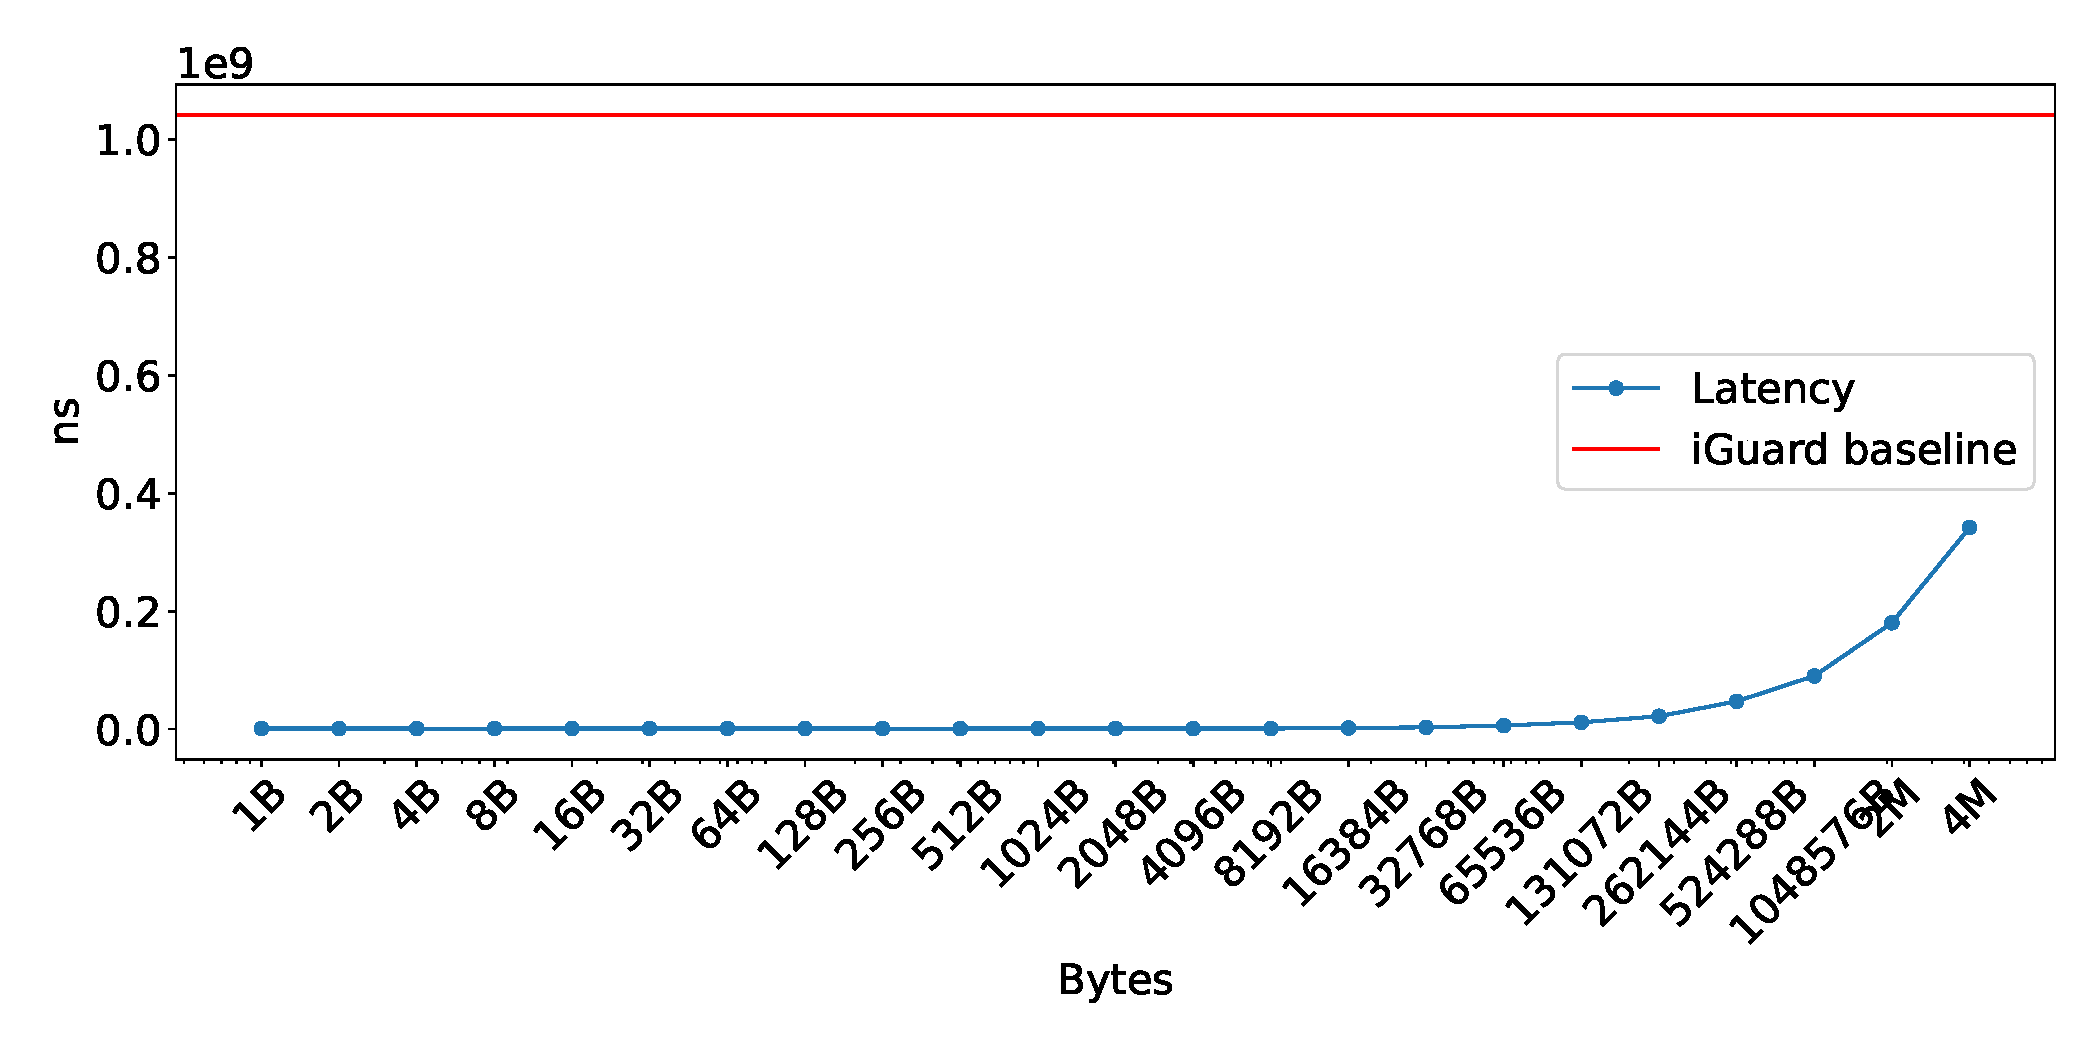
\includegraphics[width=0.5\textwidth]{img/end_to_end_latency.pdf} \caption{Runtime Overhead\xiangyu{Add more description to the figure?}} \label{fig:end_to_end_latency} \end{figure}

\begin{figure} \centering 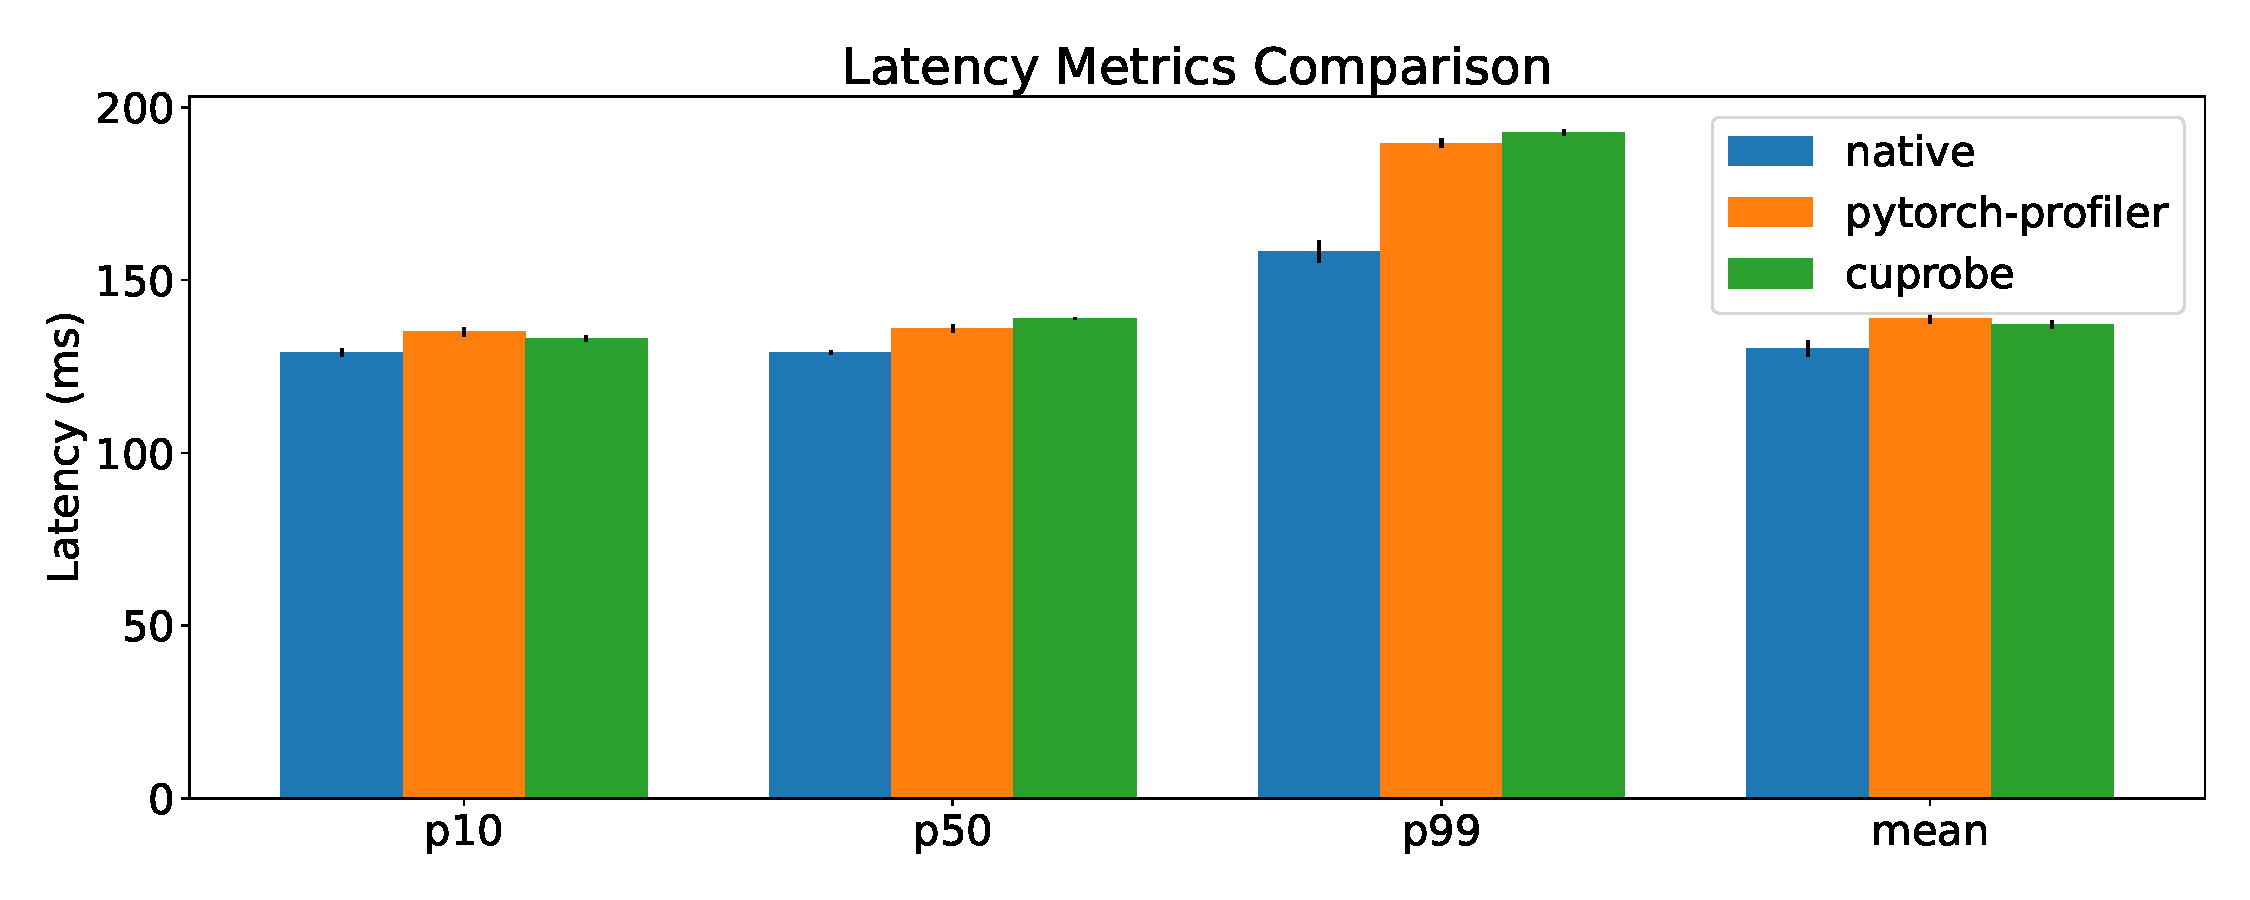
\includegraphics[width=0.5\textwidth]{img/latency_comparison.pdf} \caption{Resnet Inference Latency Overhead} \label{fig:latency1} \end{figure}

\subsection{\sys{} Performance}
We compare end-to-end throughput and time-to-result against a native baseline (no persistent kernel, no PTX injection). For small batches, \sys{} pays modest startup/JIT cost but reduces launch frequency; for larger or irregular workloads, it matches or beats native by avoiding relaunches and sustaining higher utilization.

\subsection{Shared Memory Performance}
We benchmark shared-memory bandwidth and one-way latency on three servers using a 1 GiB region and both CPU-only and GPU access patterns (GPU-to-CPU and CPU-to-GPU). Servers A/B deliver 12–18 GB/s over PCIe with 8–15 µs cross-domain latencies; Server C's coherent fabric sustains \(>100\) GB/s and \(<500\) ns round-trip, highlighting the advantage of hardware coherence for live instrumentation.

\subsection{Use Case Evaluation}\label{sec:usecase_evaluation}

\subsubsection{MemTrace}\label{sec:eval_memtrace}
We evaluate accuracy and overhead on synthetic and real kernels. A bank-conflict microbenchmark shows per-warp access patterns and conflict rates within 2\% of hardware counters. In \Cref{fig:memtrace}, instrumenting GEMM, SpMV, and a 1D stencil adds under 3\% end-to-end overhead; PTX injection remains below 50 \(\mu\)s. MemTrace also pinpointed a convolution-bank conflict that a simple padding fix resolved for a 12\% gain.
\begin{figure}
\centering
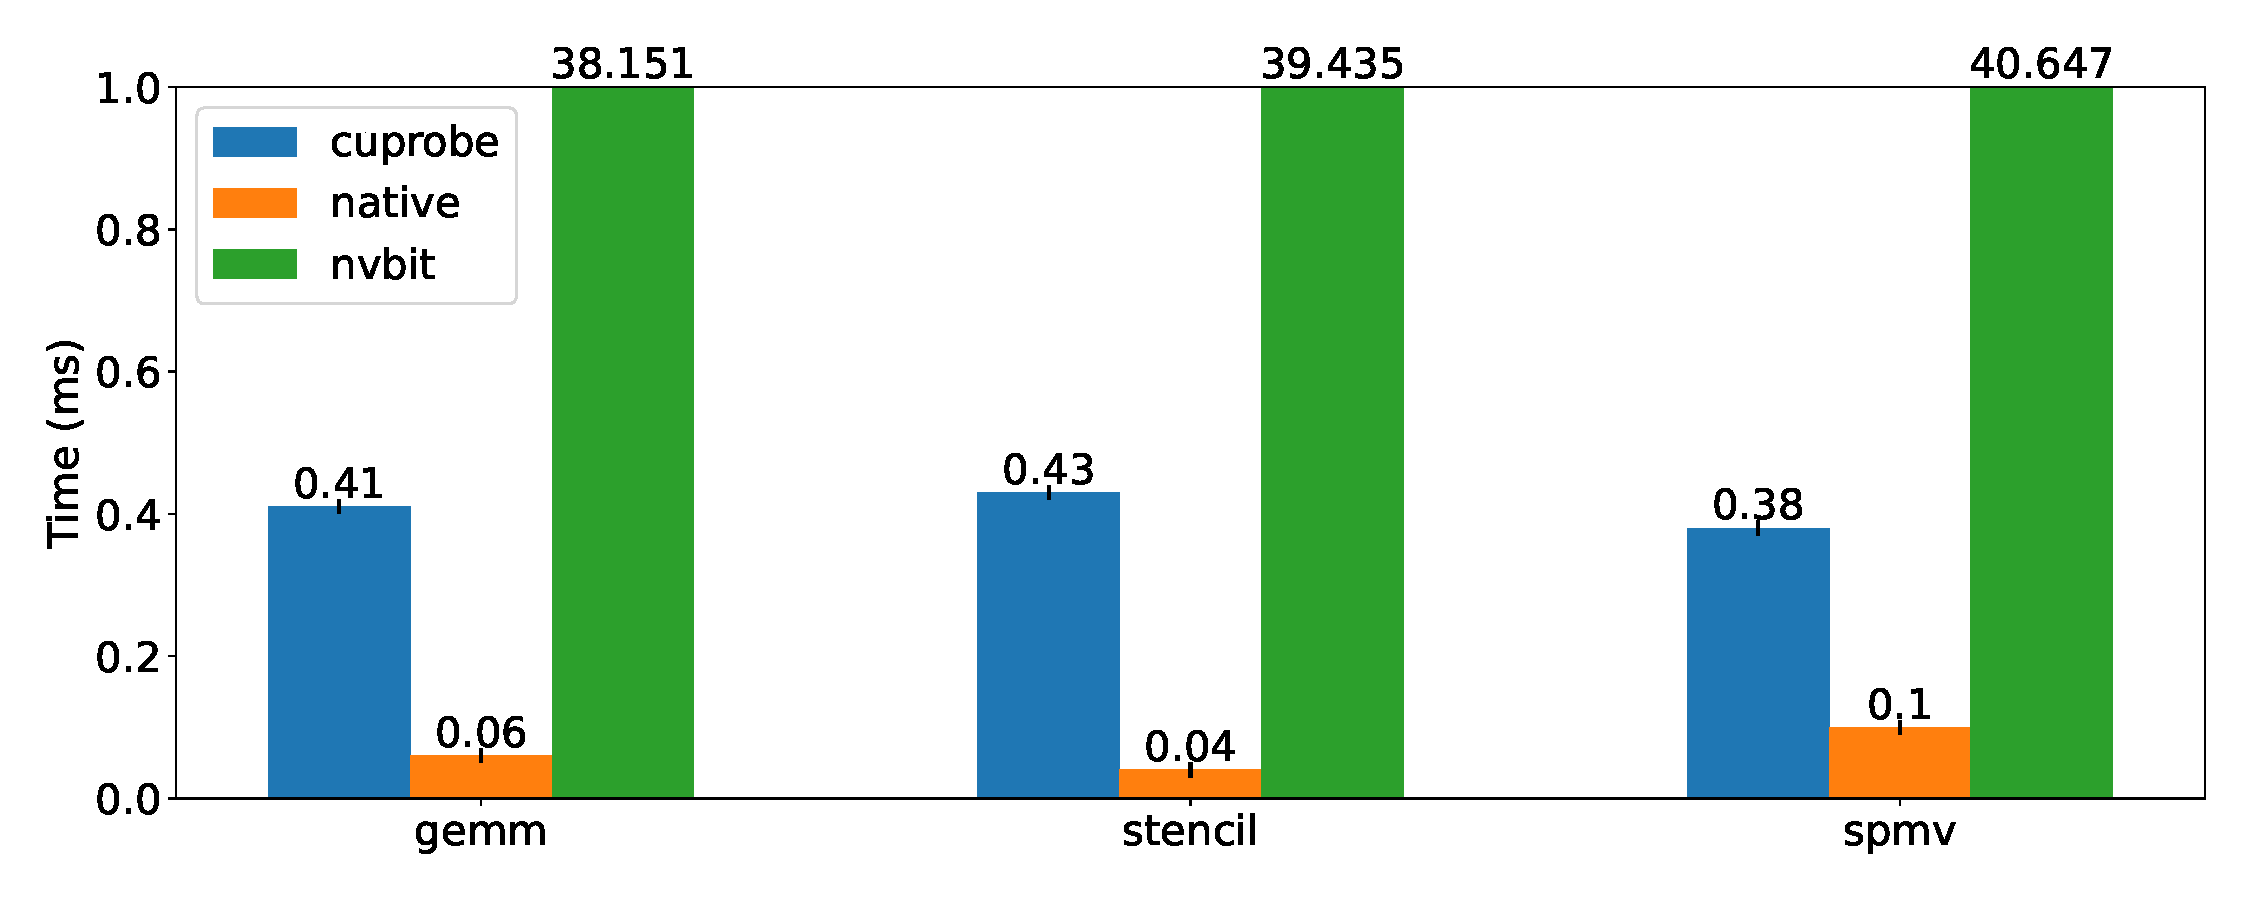
\includegraphics[width=\columnwidth]{img/memtrace.pdf}
\caption{MemTrace Overhead Comparison}\label{fig:memtrace}
\end{figure}
\subsubsection{Fair Share Scheduling}\label{sec:eval_fair_sched}

We evaluate Fair Share Scheduling in multi‐tenant scenarios where several GPU kernels with differing resource demands (compute‐bound, memory‐bound, and mixed) run concurrently on the same device. We compare three policies: (1) a naïve FIFO queue, (2) a static proportional‐share allocator that divides blocks evenly by tenant, and (3) \sys's dynamic Fair Share Scheduler, which continuously measures per‐block execution times via injected PTX trampolines and reassigns block‐launch quotas to equalize effective progress across tenants.

Experiments use ResNet-18 inference and a BFS kernel. Tenants submit 256-block batches; the host recomputes quotas every 10 ms to equalize progress. We quantify fairness using Jain's index:
\[
  F = \frac{\bigl(\sum_{i=1}^M x_i\bigr)^2}{M\,\sum_{i=1}^M x_i^2}\!,
\]
where \(x_i\) is the throughput achieved by tenant \(i\) and \(M=3\).

\Cref{fig:plot_cuda_scheduler} compares FIFO, Static Proportional, and Fair Share on runtime (blue, left axis) and launch latency (orange, right axis). FIFO: ~205 s and ~1 ms; Static: ~130 s and ~0.6 ms but higher variance; Fair Share: ~122 s and ~0.5 ms with tighter error bars. Adaptive quotas improve both throughput and stability over baselines.


\begin{figure}
\centering
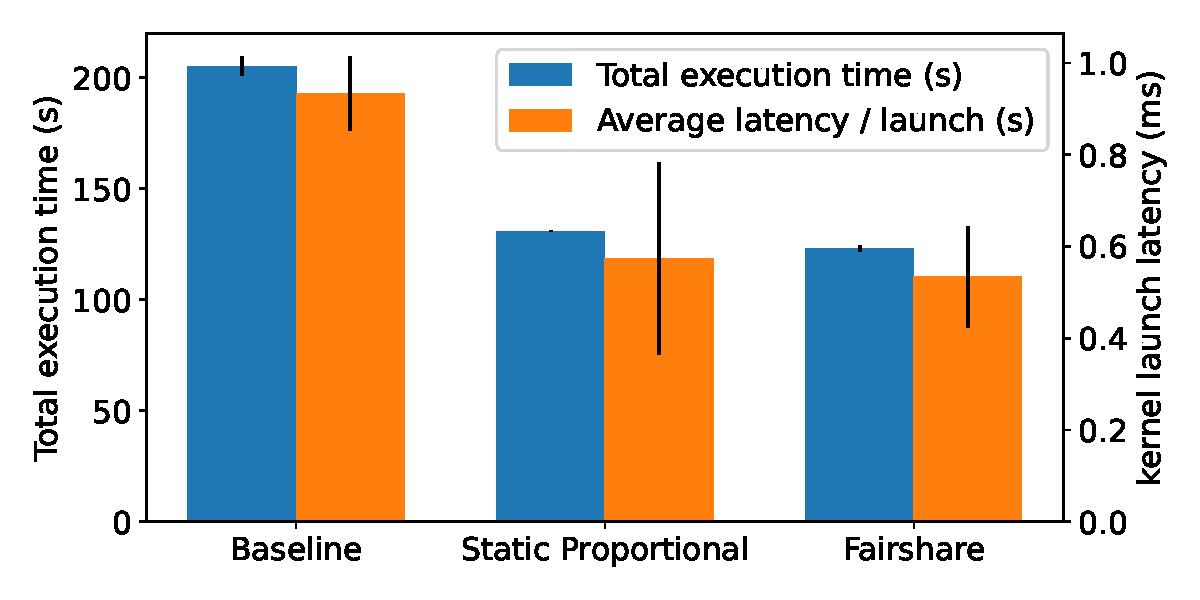
\includegraphics[width=\columnwidth]{img/plot_cuda_scheduler.pdf}
\caption{BFS Scheduler Comparison}\label{fig:plot_cuda_scheduler}
\end{figure}

\subsubsection{ML Green: CPU–GPU Collaborative Inference}\label{sec:eval_ml_green}
We integrate \sys into ResNet-50 and LLaMA2 pipelines on H100+CXL and compare: (1) static CPU–GPU splits, (2) online profiling with LRU/LFU caching, and (3) full CPU and full GPU offloading.

\paragraph{Static CPU–GPU splitted inference}
\Cref{fig:slicing-percentage} shows that offloading deeper ResNet/LLaMA2 layers reduces tail latency by 15–40\% versus CPU-only until GPU occupancy and memory bandwidth saturate (plateauing around 20–25 slices). Gains stem from efficient GEMM/conv/attention on tensor cores; very small models may not benefit.

\Cref{fig:heatmap,fig:heatmap1} plot LLaMA2 latencies over split points. Latency drops as more layers move to GPU, with the pure-GPU case best (0.323 s vs. 0.347 s for the best two-way split). Server A ranges ~9.12–9.15 s (mixed), Server B ~0.5–8 s. Beyond ~20–25 offloaded layers, launch overheads and bandwidth saturation limit gains.

\paragraph{Optimized online profiling and LRU or LFU caching policy}
For online optimization, \sys collects per-layer times, transfer latencies, and cache stats, then periodically selects the latency-minimizing split while balancing CPU/GPU load. A small shared "partition cache" (LRU/LFU) stores compiled snippets and deltas, keeping overhead under 2\% and delivering 10–12\% throughput gains over static splits as workloads evolve.

\paragraph{Full CPU Full GPU offloading}
\Cref{fig:power_vs_throughput} overlays renewable generation and token throughput for two pipelines (Tok1: full-CPU/full-GPU offloading; Tok2: GPU frequency scaling). Throughput tracks solar/wind availability, peaking at ~1.35–1.40 tok/s and returning to ~0.8 tok/s overnight; Tok2 maintains a small advantage (\(~0.05\) tok/s). This illustrates energy-aware scheduling benefits without exceeding power budgets.

\xiangyu{Is it possible for us to expand the impact of \sys{} by mentioning its potential to target more use cases.}

\begin{figure}
\centering
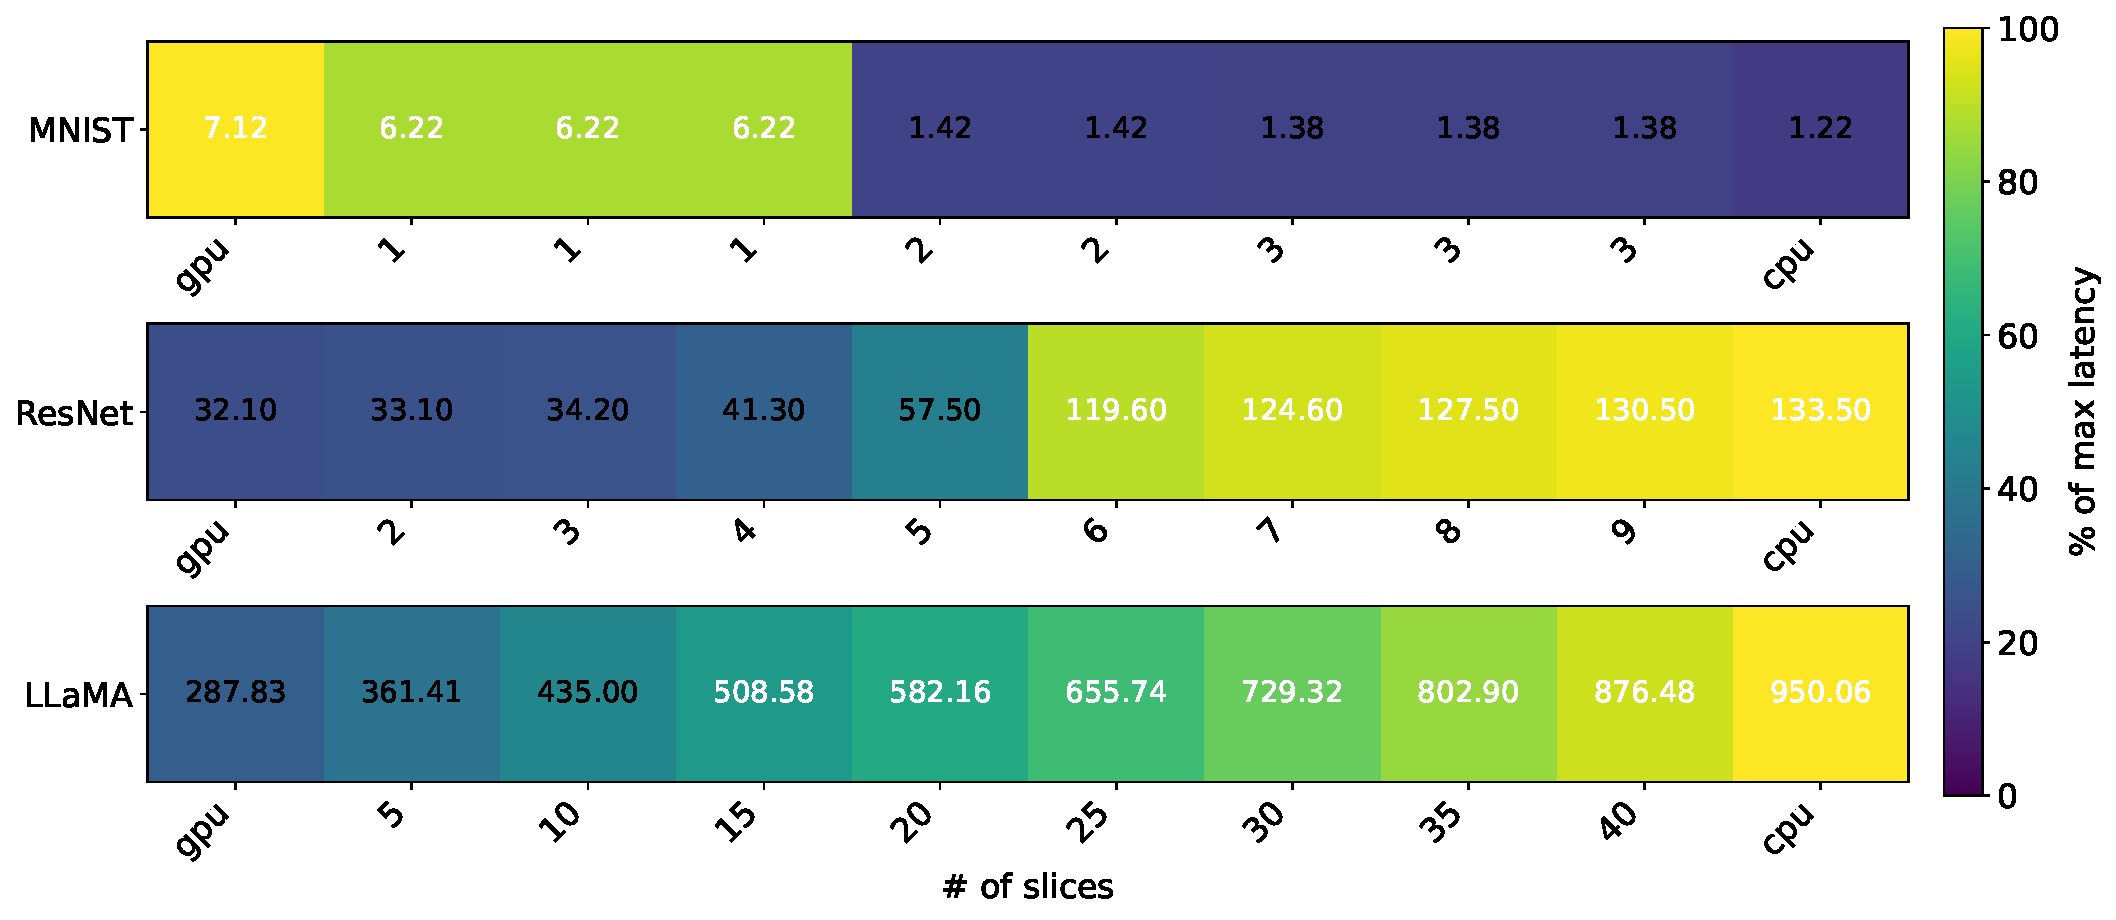
\includegraphics[width=\columnwidth]{img/slice_plot.pdf}
\caption{Latency comparison of static CPU GPU slice percentage}\label{fig:slicing-percentage}
\end{figure}
\begin{figure}
\centering
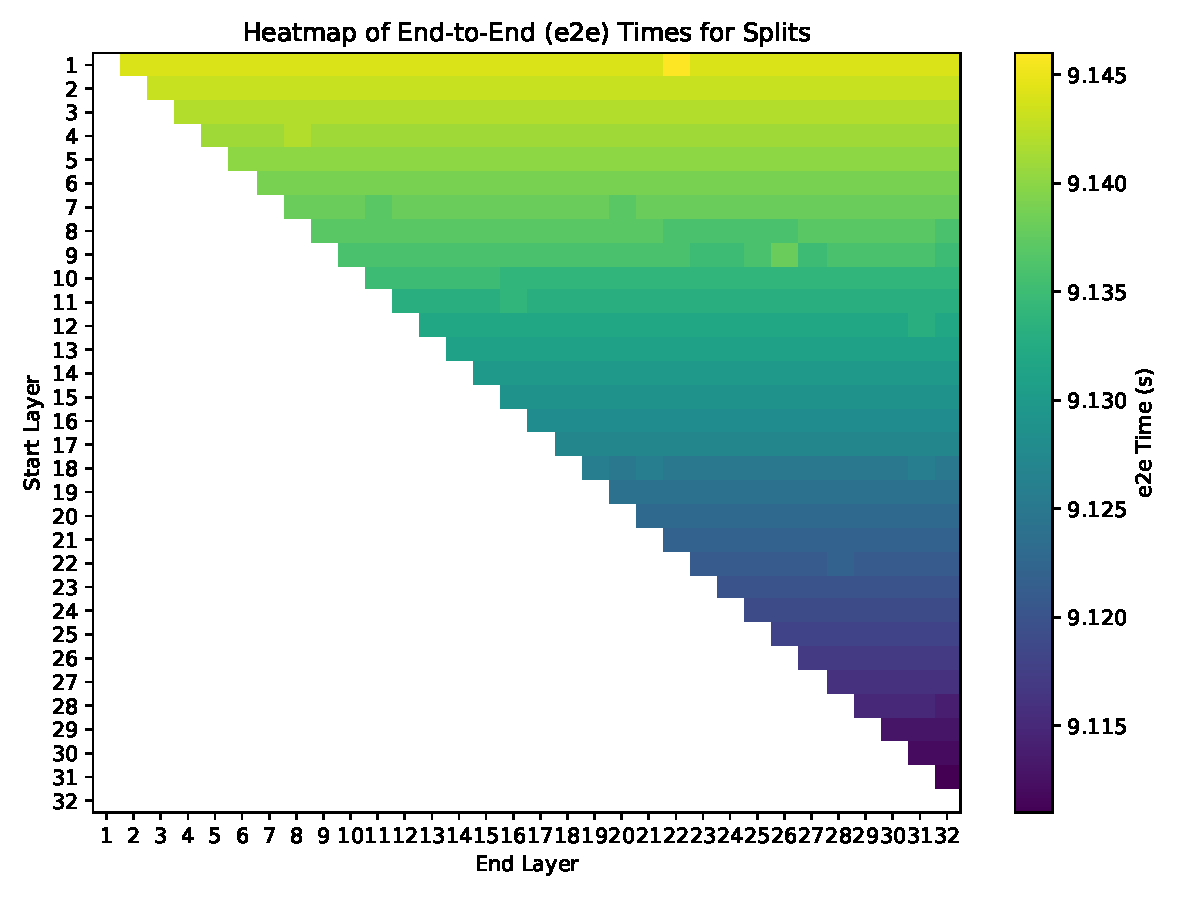
\includegraphics[width=\columnwidth]{img/heatmap.pdf}
\caption{LLAMA2 hidden representation Heatmap on Server A}\label{fig:heatmap}
\end{figure}
\begin{figure}
\centering
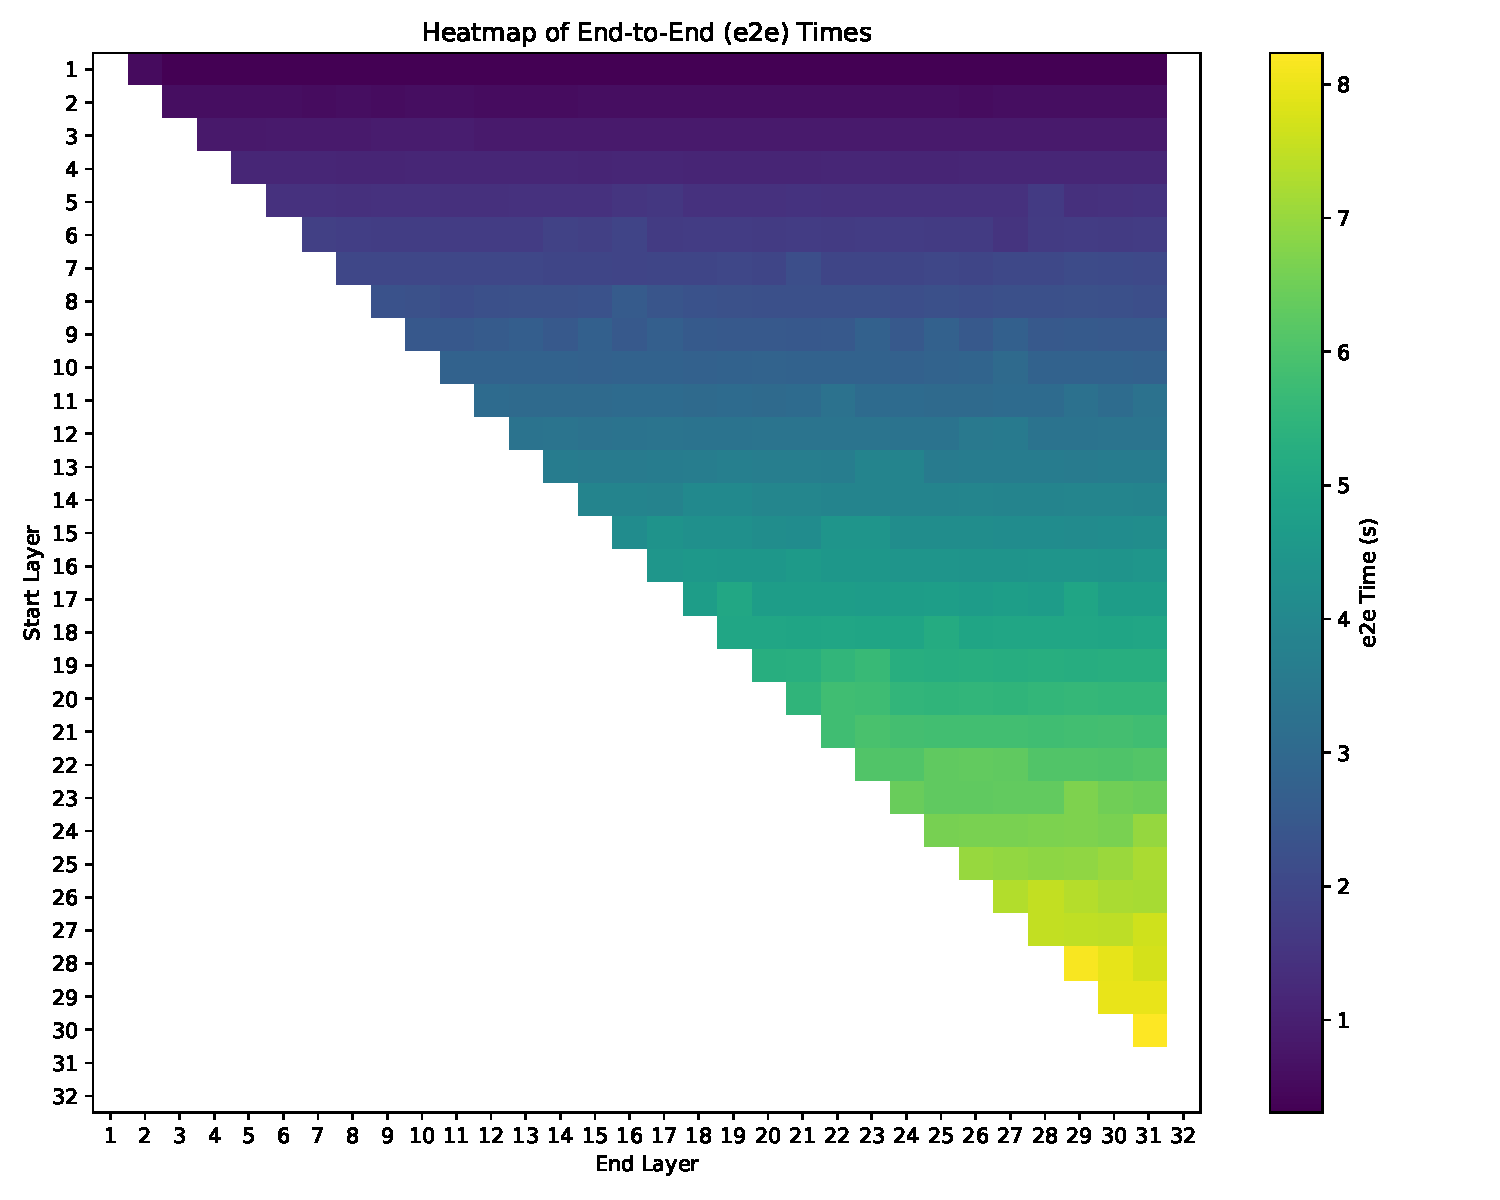
\includegraphics[width=\columnwidth]{img/heatmap1.pdf}
\caption{LLAMA2 hidden representation Heatmap on Server B}\label{fig:heatmap1}
\end{figure}
\begin{figure}
\centering
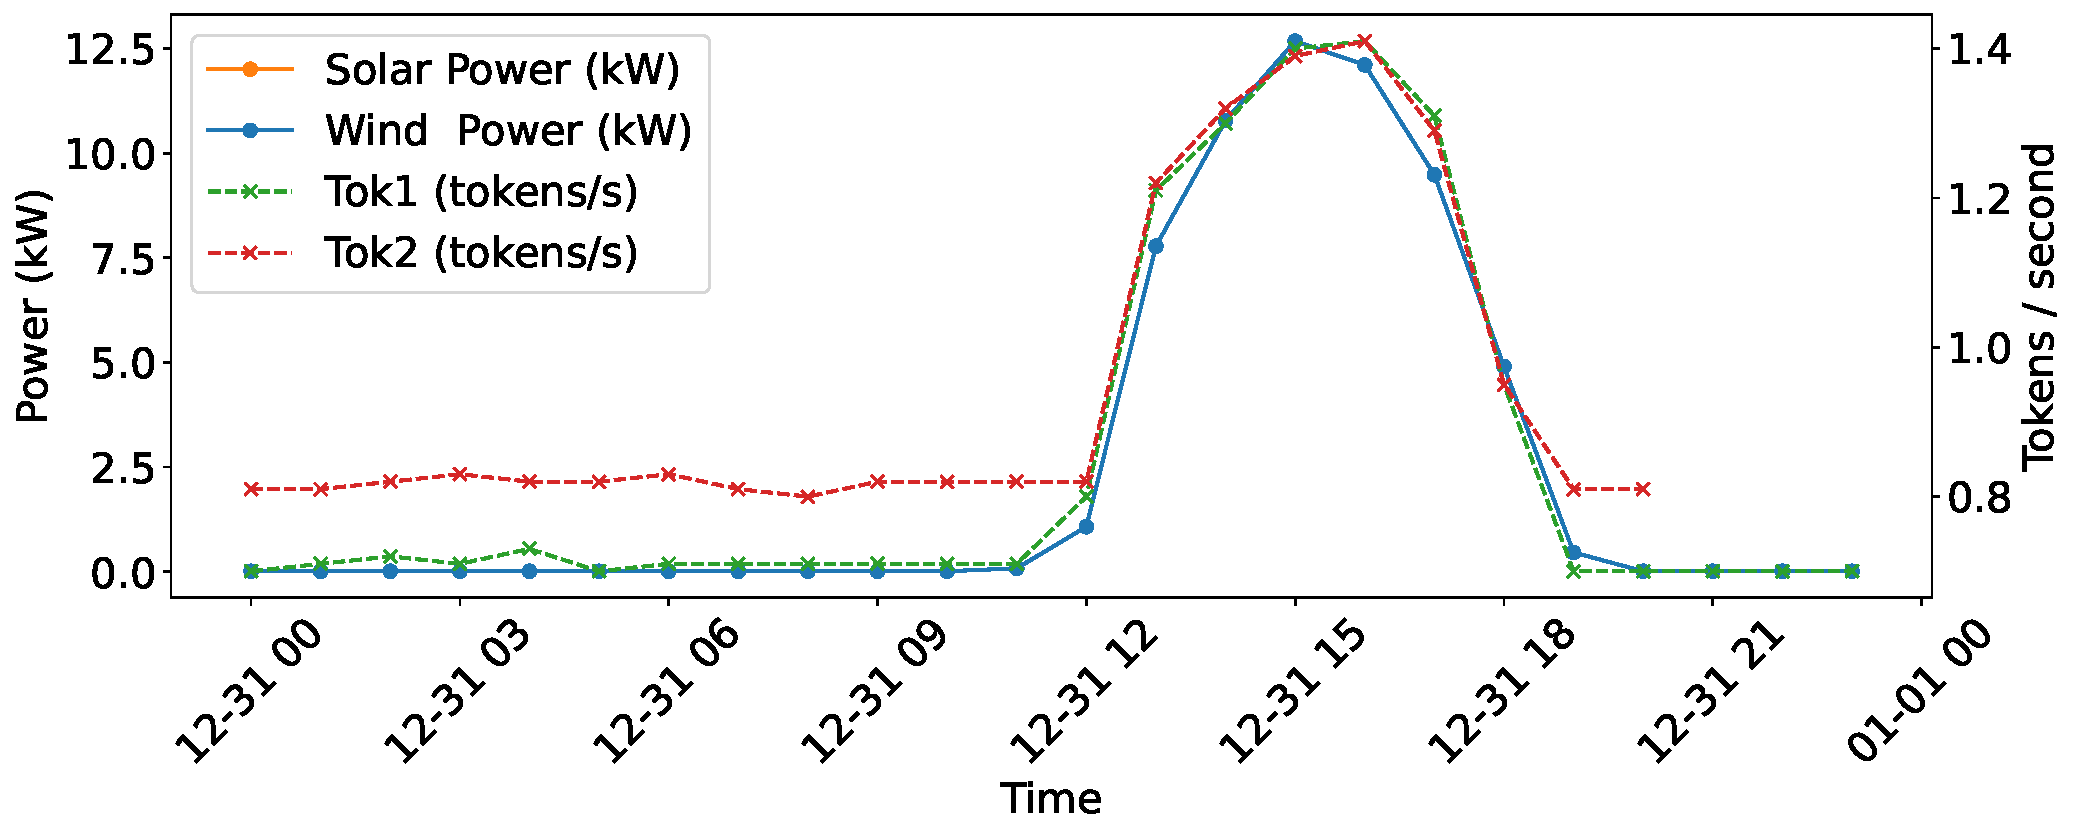
\includegraphics[width=\columnwidth]{img/plot_data.pdf}
\caption{LLAMA2 Power Generation Full CPU Full GPU offload on 2015‑12‑31}\label{fig:power_vs_throughput}
\end{figure}
